\documentclass[10pt]{article}
\usepackage[utf8]{inputenc}
\usepackage[spanish]{babel}
\usepackage{amsmath}
\usepackage{amsfonts}
\usepackage{amssymb}
\usepackage{graphics}
\usepackage{graphicx}
\usepackage[left=2cm,right=2cm,top=2cm,bottom=2cm]{geometry}
\usepackage{imakeidx}
\makeindex[columns=3, title=Alphabetical Index, intoc]
\usepackage{listings}
\usepackage{xcolor}
\usepackage{multicol}
\usepackage{changepage}
\usepackage{float}
\usepackage{cite}
\usepackage{url}
\usepackage{hyperref}
\usepackage[document]{ragged2e}
\usepackage{pdfpages}
\usepackage{lscape}

\hypersetup{
    colorlinks=true,
    linkcolor=blue,
    filecolor=magenta,
    urlcolor=blue,
}

\definecolor{codegreen}{rgb}{0,0.6,0}
\definecolor{codegray}{rgb}{0.5,0.5,0.5}
\definecolor{codepurple}{rgb}{0.58,0,0.82}
\definecolor{backcolour}{rgb}{0.95,0.95,0.92}

\lstdefinestyle{mystyle}{
    backgroundcolor=\color{backcolour},
    commentstyle=\color{codegreen},
    keywordstyle=\color{magenta},
    numberstyle=\tiny\color{codegray},
    stringstyle=\color{codepurple},
    basicstyle=\ttfamily\footnotesize,
    breakatwhitespace=false,
    breaklines=true,
    captionpos=b,
    keepspaces=true,
    numbers=left,
    numbersep=5pt,
    showspaces=false,
    showstringspaces=false,
    showtabs=false,
    tabsize=3
}

\lstset{style=mystyle}

\title{Centro de Investigación en Cómputo\\Instituto Politécnico Nacional\\Metaheurísticas\\Actividad No. 5\\ Solución de problemas mediante Ascensión de Colinas}

\author{Por: Adrian González Pardo}

\date{\today}

\newcommand\tab[1][1cm]{\hspace*{#1}}

\begin{document}
\maketitle
\section{Funciones a optimizar}
\begin{center}
  \begin{tabular}{|c|c|}
    \hline
    Función a evaluar & Forma o descripción de la función\\
    \hline
    Alpine Function & \(\displaystyle f_{1}(x)=\sum_{i=1}^{D} \left|x_{i}\sin(x_{i})+0.1x_{i}\right|\) \\
    \hline
    Dixon \& Price Function & \(\displaystyle f_{2}(x)=(x_{1}-1)^{2}\sum_{i=2}^{D} i\left(2\sin(x_{i})-x_{i-1}\right)^{2}\)\\
    \hline
    Quintic Function & \(\displaystyle f_{3}(x)=\sum_{i=1}^{D} \left|x_{i}^{5}-3x_{i}^{4}+4x_{i}^3-2x_{i}^{2}-10x_{i}-4\right|\)\\
    \hline
    Schwefel 2.23 Function & \(\displaystyle f_{4}(x)=\sum_{i=1}^{D}x_{i}^{10}\)\\
    \hline
    Streched V Sine Wave Function & \(\displaystyle f_{5}(x)=\sum_{i=1}^{D-1}(x_{i+1}^{2}+x_{i}^{2})^{0.25}\left[\sin^{2}\left\{50(x_{i+1}^{2}+x_{i}^{2})^{0.1}\right\}+1\right]\)\\
    \hline
    Sum Squares Function & \(\displaystyle f_{6}(x)=\sum_{i=1}^{D}ix_{i}^{2}\)\\
    \hline
  \end{tabular}
\end{center}
\clearpage
\section{Código de implementación}
El código fue implementado en lenguaje Ruby para el cálculo de las funciones en $D$ dimensiones y a traves de 1 indice se determina la selección de que función se trabajara.
\subsection{Función que selecciona que $f(x)$ trabajara}
\begin{center}
  \lstinputlisting[language=Ruby]{funcion0.rb}
\end{center}
\subsection{Función Alpine}
\begin{center}
  \lstinputlisting[language=Ruby]{funcion1.rb}
\end{center}

\subsection{Función Dixon \& Price}
\begin{center}
  \lstinputlisting[language=Ruby]{funcion2.rb}
\end{center}

\subsection{Función Quintic}
\begin{center}
  \lstinputlisting[language=Ruby]{funcion3.rb}
\end{center}

\subsection{Función Schwefel}
\begin{center}
  \lstinputlisting[language=Ruby]{funcion4.rb}
\end{center}

\subsection{Función Streched}
\begin{center}
  \lstinputlisting[language=Ruby]{funcion5.rb}
\end{center}

\subsection{Función Sum Squares}
\begin{center}
  \lstinputlisting[language=Ruby]{funcion6.rb}
\end{center}

\section{Tabla de resultados}


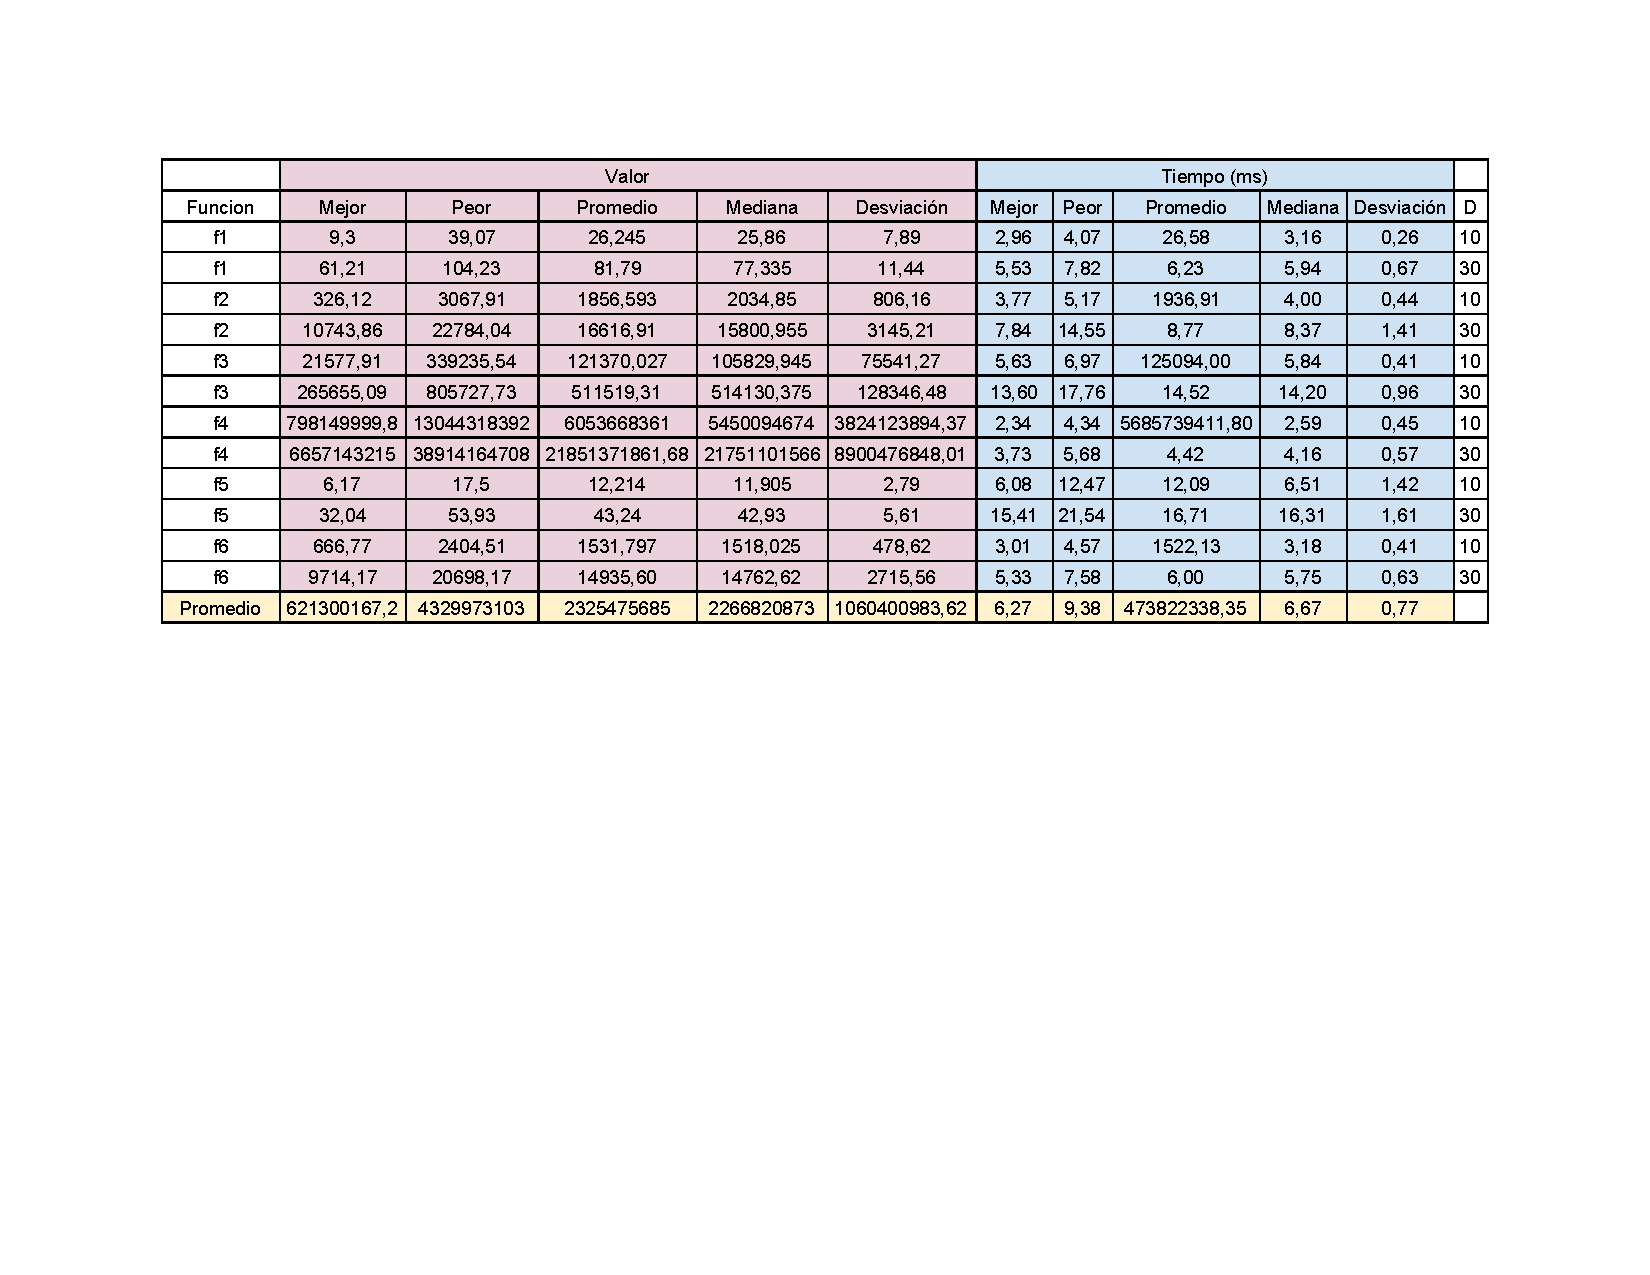
\includepdf[pages=-]{../funciones_min.pdf}
\end{document}
